% !TEX root = main.tex
\section{Production and Detection Asymmetries}

\subsection{$B_s$ Production Asymmetry}
\label{sec:productionAsym}

The production rates of $b$ and $\bar b$ hadrons in $pp$ collisions are not expected to be identical,
therefore this effect must be taken into account when computing CP asymmetries.
The production asymmetry for $B_s$ mesons is defined as:
\begin{equation}
	A_p(B_s^0) = \frac{\sigma(\bar B_s^0) - \sigma(B_s^0)}{\sigma(\bar B_s^0) + \sigma(B_s^0)}
\end{equation}
where $\sigma$ are the corresponding production cross-section.
This asymmetry was
measured by LHCb in $pp$ collisions at $\sqrt s = 7 \tev$ and  $\sqrt s = 8 \tev$ 
by means of a time-dependent analysis of $B_s \to D_s^- \pip$ decays \cite{Aaij:2017mso}.
The results in bins of $p_T$ and $\eta$ of the $B_s$ meson  are shown in Table \ref{tab:Ap}.
To correct for the different kinematics of $B_s \to D_s^- \pip$ and
$\Bs\to\Ds\kaon\pion\pion$ decays, the measured $B_s$ production asymmetries $A_p(p_T,\eta)$ 
are folded with the \textsf{sWeighted} $p_T,\eta$ distribution of our signal channel.
The resulting effective production asymmetries are:
\begin{align}
	A_p(B_s^0)_{2011} &= (-0.506 \pm 1.90 ) \% \\
	A_p(B_s^0)_{2012} &= (\phantom{-}0.164 \pm 1.30 ) \% \\
	A_p(B_s^0)_{\text{Run-I}} &= (-0.045 \pm 1.04 ) \% .
\end{align}
As for Run-II data no measurement is available yet, we determine the production asymmetry from $B_s \to D_s\pi\pi\pi$ data together
with the tagging parameters.
 
%Production asymmetries for year = 11
%Normalization channel: 
%Asymmetry = -0.00210574 +/- 0.0189955
%Signal channel: 
%Asymmetry = -0.00506342 +/- 0.0187838
%
%Production asymmetries for year = 12
%Normalization channel: 
%Asymmetry = 0.00471172 +/- 0.0129602
%Signal channel: 
%Asymmetry = 0.00164359 +/- 0.0124882
%
%Combined Asymmetry (Norm) = 0.00271833 +/- 0.0107215
%Combined Asymmetry (Signal) = -0.000450934 +/- 0.0104004

\begin{table}[h]
\caption{$B_s$ production asymmetries in kinematic bins for 2011 and 2012 data. \cite{Aaij:2017mso}}
\centering
\begin{tabular}{c c c c}
\mbox{$p_{\rm T}$}\xspace [ $ {\mathrm{\,Ge\kern -0.1em V\!/}c}$ \xspace] & $\eta$ & $A_{\rm P}( B\xspace\xspace^0_ s\xspace\xspace\xspace)_{\sqrt{s}\xspace = 7\, \mathrm{\,Te\kern -0.1em V}\xspace}$ & $A_{\rm P}( B\xspace\xspace^0_ s\xspace\xspace\xspace)_{\sqrt{s}\xspace = 8\, \mathrm{\,Te\kern -0.1em V}\xspace}$ \\
\hline
$(2.00,   7.00)$   &  $(2.10,  3.00)$  &  $  \phantom{-}0.0166  \pm  0.0632  \pm  0.0125  $  &  $  \phantom{-}0.0412  \pm  0.0416  \pm  0.0150  $     \\
$(2.00,   7.00)$   &  $(3.00,  3.30)$  &  $  \phantom{-}0.0311  \pm  0.0773  \pm  0.0151  $  &  $  -0.0241            \pm  0.0574  \pm  0.0079  $    \\
$(2.00,   7.00)$   &  $(3.30,  4.50)$  &  $  -0.0833            \pm  0.0558  \pm  0.0132  $     &  $  \phantom{-}0.0166  \pm  0.0391  \pm  0.0092  $        \\
$(7.00,   9.50)$   &  $(2.10,  3.00)$  &  $  \phantom{-}0.0364  \pm  0.0479  \pm  0.0068  $   &  $  \phantom{-}0.0482  \pm  0.0320  \pm  0.0067  $   \\
$(7.00,   9.50)$   &  $(3.00,  3.30)$  &  $  \phantom{-}0.0206  \pm  0.0682  \pm  0.0127  $ &  $  \phantom{-}0.0983  \pm  0.0470  \pm  0.0155  $     \\
$(7.00,   9.50)$   &  $(3.30,  4.50)$  &  $  \phantom{-}0.0058  \pm  0.0584  \pm  0.0089  $  &  $  -0.0430            \pm  0.0386  \pm  0.0079  $   \\
$(9.50,   12.00)$  &  $(2.10,  3.00)$  &  $  -0.0039            \pm  0.0456  \pm  0.0121  $      &  $  \phantom{-}0.0067  \pm  0.0303  \pm  0.0063  $     \\
$(9.50,   12.00)$  &  $(3.00,  3.30)$  &  $  \phantom{-}0.1095  \pm  0.0723  \pm  0.0179  $  &  $  -0.1283            \pm  0.0503  \pm  0.0171  $     \\
$(9.50,   12.00)$  &  $(3.30,  4.50)$  &  $  \phantom{-}0.1539  \pm  0.0722  \pm  0.0212  $  &  $  -0.0500            \pm  0.0460  \pm  0.0104  $  \\
$(12.00,  30.00)$  &  $(2.10,  3.00)$  &  $  -0.0271            \pm  0.0336  \pm  0.0061  $  &  $  -0.0012            \pm  0.0222  \pm  0.0050  $        \\
$(12.00,  30.00)$  &  $(3.00,  3.30)$  &  $  -0.0542            \pm  0.0612  \pm  0.0106  $    &  $  \phantom{-}0.0421  \pm  0.0416  \pm  0.0162  $     \\
$(12.00,  30.00)$  &  $(3.30,  4.50)$  &  $  -0.0586            \pm  0.0648  \pm  0.0150  $     &  $  \phantom{-}0.0537  \pm  0.0447  \pm  0.0124  $      \\
\end{tabular}
\label{tab:Ap}
\end{table}

\clearpage
\subsection{$\Km\pip$ Detection Asymmetry}
\label{sec:KpiAsym}

The presented measurement of the CKM-angle $\gamma$ using $\Bs\to\Ds\kaon\pion\pion$ decays is sensitive to a possible charge asymmetry of the kaon. 
Kaons are known to have a nuclear cross-section which is asymmetrically dependent on the sign of their charge. 
It is indispensable to determine the charge asymmetry of the kaon, as fitting without taking this effect into account would introduce a 'fake' CP violation. 
Instead of determining the single track detection asymmetry of a kaon, it is found that the combined two track asymmetry of a kaon-pion pair is much easier to access \cite{Gordon:1482647} . 
Therefore, the two track asymmetry defined as 
\begin{equation}
A^{det}(\Km\pip) = \frac{\epsilon^{det}(\Km\pip) -\epsilon^{det}(\Kp\pim)}{\epsilon^{det}(\Km\pip) + \epsilon^{det}(\Kp\pim)},
\label{eq:KpiDetAsymDef}
\end{equation}

is used.

%$A^{det}(\Km\pip$) can further be expressed, assuming no CP violation in Cabbibo-favoured charm modes, 
This asymmetry can be measured from the difference in asymmetries in the $\Dp\to\Km\pip\pip$ and $\Dp\to\KS\pip$ modes
% from Cabbibo-favoured charm calibration modes (assuming no CP violation)
\cite{Davis:2310213}:
\begin{equation}
\begin{split}
A^{det}(\Km\pip) = & \frac{N(\Dp\to\Km\pip\pip) - N(\Dm\to\Kp\pim\pim)}{N(\Dp\to\Km\pip\pip) + N(\Dm\to\Kp\pim\pim)} \\
                  & - \frac{N(\Dp\to\KS\pip) - N(\Dm\to\KS\pim)}{N(\Dp\to\KS\pip) + N(\Dm\to\KS\pim)} \\
                  & - A(\Kz),
\end{split}
\label{eq:KpiDetAsymDef}
\end{equation}
where possible CP violation in the $\Dp\to\KS\pip$ mode is predicted to be smaller than $10^{-4}$ in the Standard Model \cite{Bigi:1994aw}.
%Using Eq. \ref{eq:KpiDetAsymDef}, the two track $\Km\pip$ asymmetry is obtained from the difference in asymmetries in the $\Dp\to\Km\pip\pip$ and $\Dp\to\KS\pip$ modes. 
The asymmetry in the neutral kaon system, $A(\Kz)$, has to be taken into account as a correction. 

We use a dedicated LHCb tool to determine $A^{det}(\Km\pip)$ for all data taking periods used in this analysis. A detailed description can be found in \cite{Davis:2310213}.
The tool provides large calibration samples of $\Dpm\to\Kpm\pipm\pipm$ and $\Dpm\to\KS\pipm$ decays, which are used to determine the asymmetry following Eq. \ref{eq:KpiDetAsymDef}. 
Several weighting steps are performed to match the kinematics of the calibration samples to our signal decay sample: 

First, weights are assigned to the $\Kpm$ and $\pipm$ of the $\Dpm\to\Kpm\pipm\pipm$ sample, using $\ptot$, $\eta$ of the $\Kpm$ and $\pt$, $\eta$ of the $\pipm$ from our $\Bs\to\Ds\kaon\pion\pion$ signal decay.
Then, weights are assigned to the $\Dpm$ ($\pt, \eta$) and the $\pipm$ ($\pt$) of the $\Dpm\to\KS\pipm$ sample to match the corresponding, weighted distributions of the $\Dpm\to\Kpm\pipm\pipm$ sample.
In a last step, weights are assigned to match the bachelor pions $\phi$ distributions between the two calibration samples.

After the samples are weighted, fits are performed to the invariant $m(\Km\pip\pip)$/$m(\Kp\pim\pim)$ and $m(\KS\pip)$/$m(\KS\pim)$ distributions to determine $A^{det}(\Km\pip)$. 
The PDFs used to describe the invariant mass distributions consist of gaussian functions for the signal component and exponentials describing the residual background.

The detection asymmetry is determined separately for every year and (since it is a charge asymmetry effect) magnet polarity. 
Serving as an example for Run-I and Run-II, the fits used to determine $N(\Dp\to\Km\pip\pip)$/$N(\Dm\to\Kp\pim\pim)$ and $N(\Dp\to\KS\pip)$/$N(\Dm\to\KS\pim)$ 
for 2011, magnet up data and 2015, magnet up data are shown in Fig.~\ref{fig:KpiAsymFitsRun1} and \ref{fig:KpiAsymFitsRun2} respectively.
The obtained values of $A^{det}(\Km\pip)$ + $A(\Kz)$ for all years and polarities are shown in Table \ref{table:KpiDetectionAsym}.

\begin{figure}[hp]
\centering
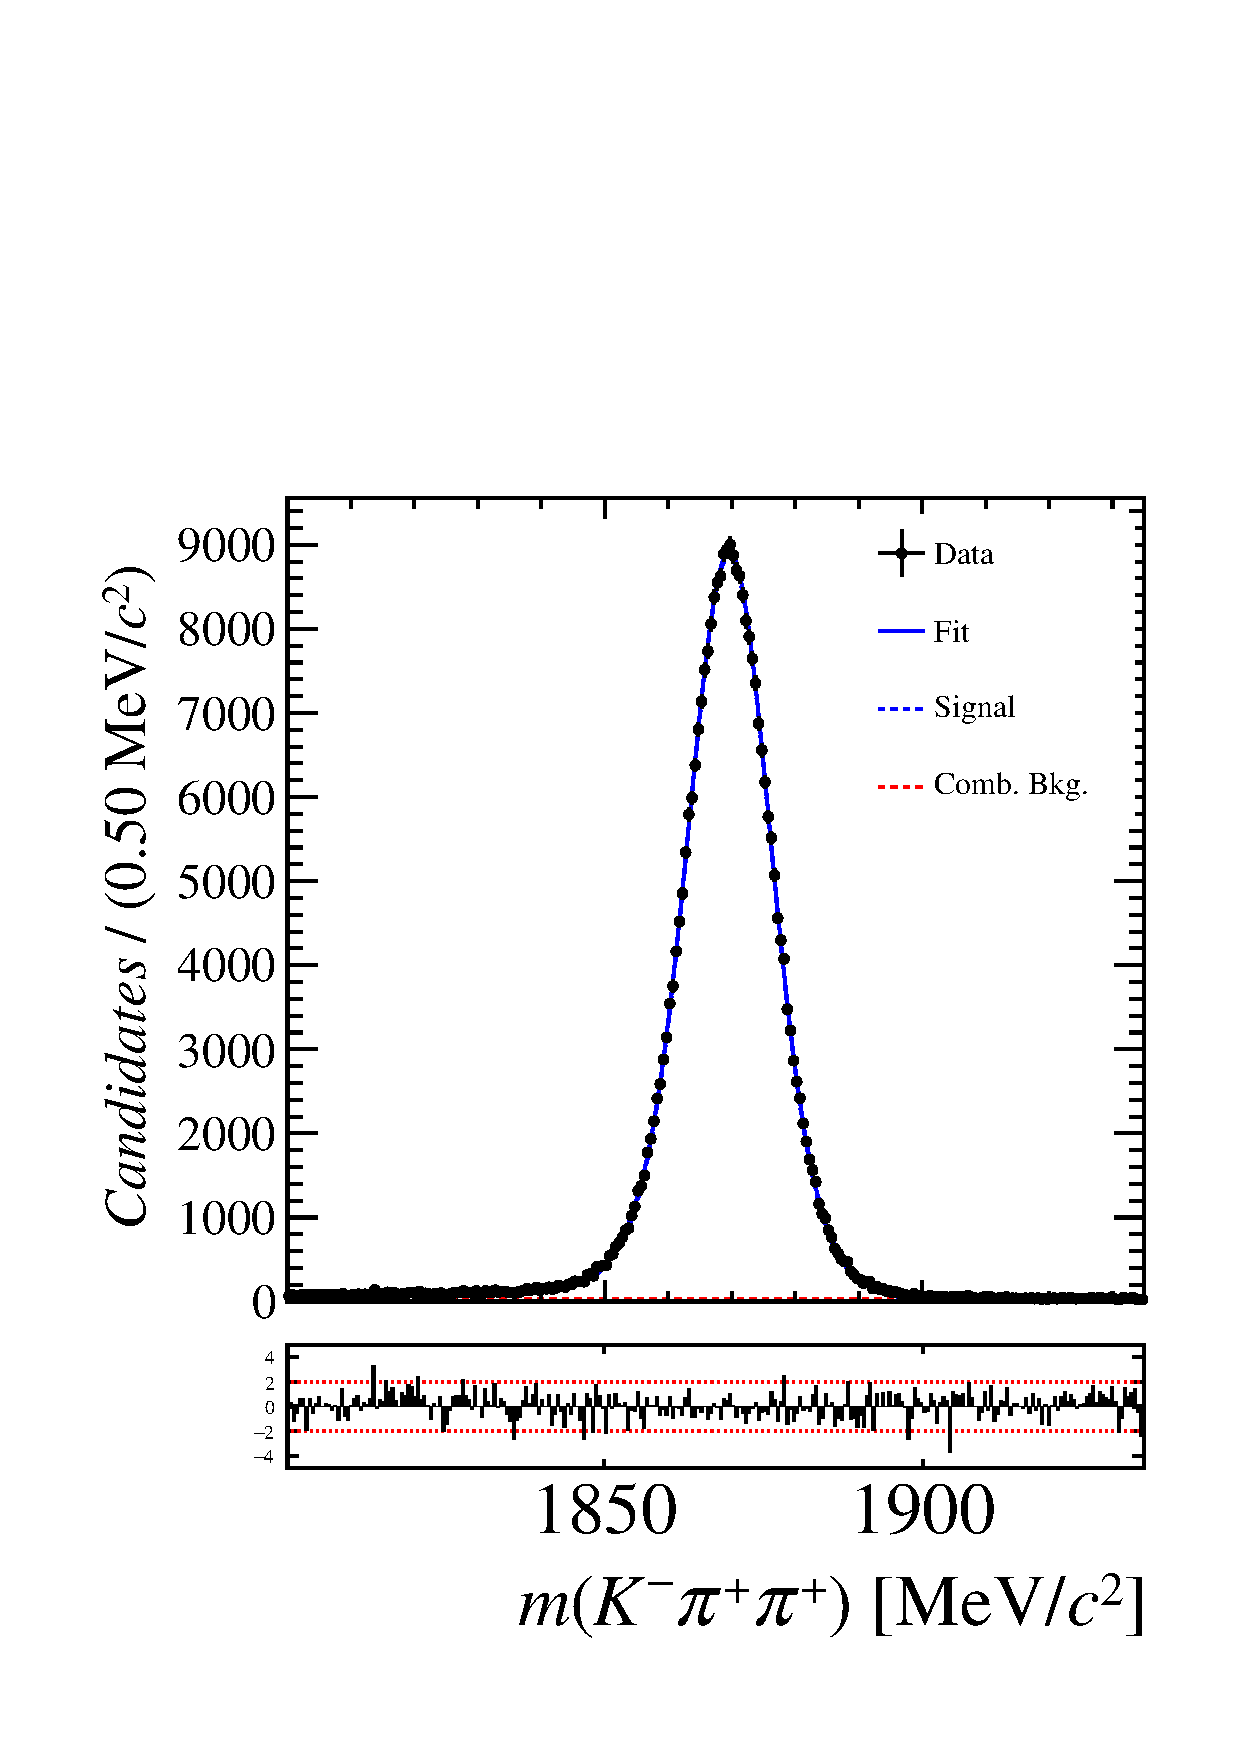
\includegraphics[height=5cm,width=0.4\textwidth]{figs/KpiAsym/fit_negative_kpipi_11up.pdf}
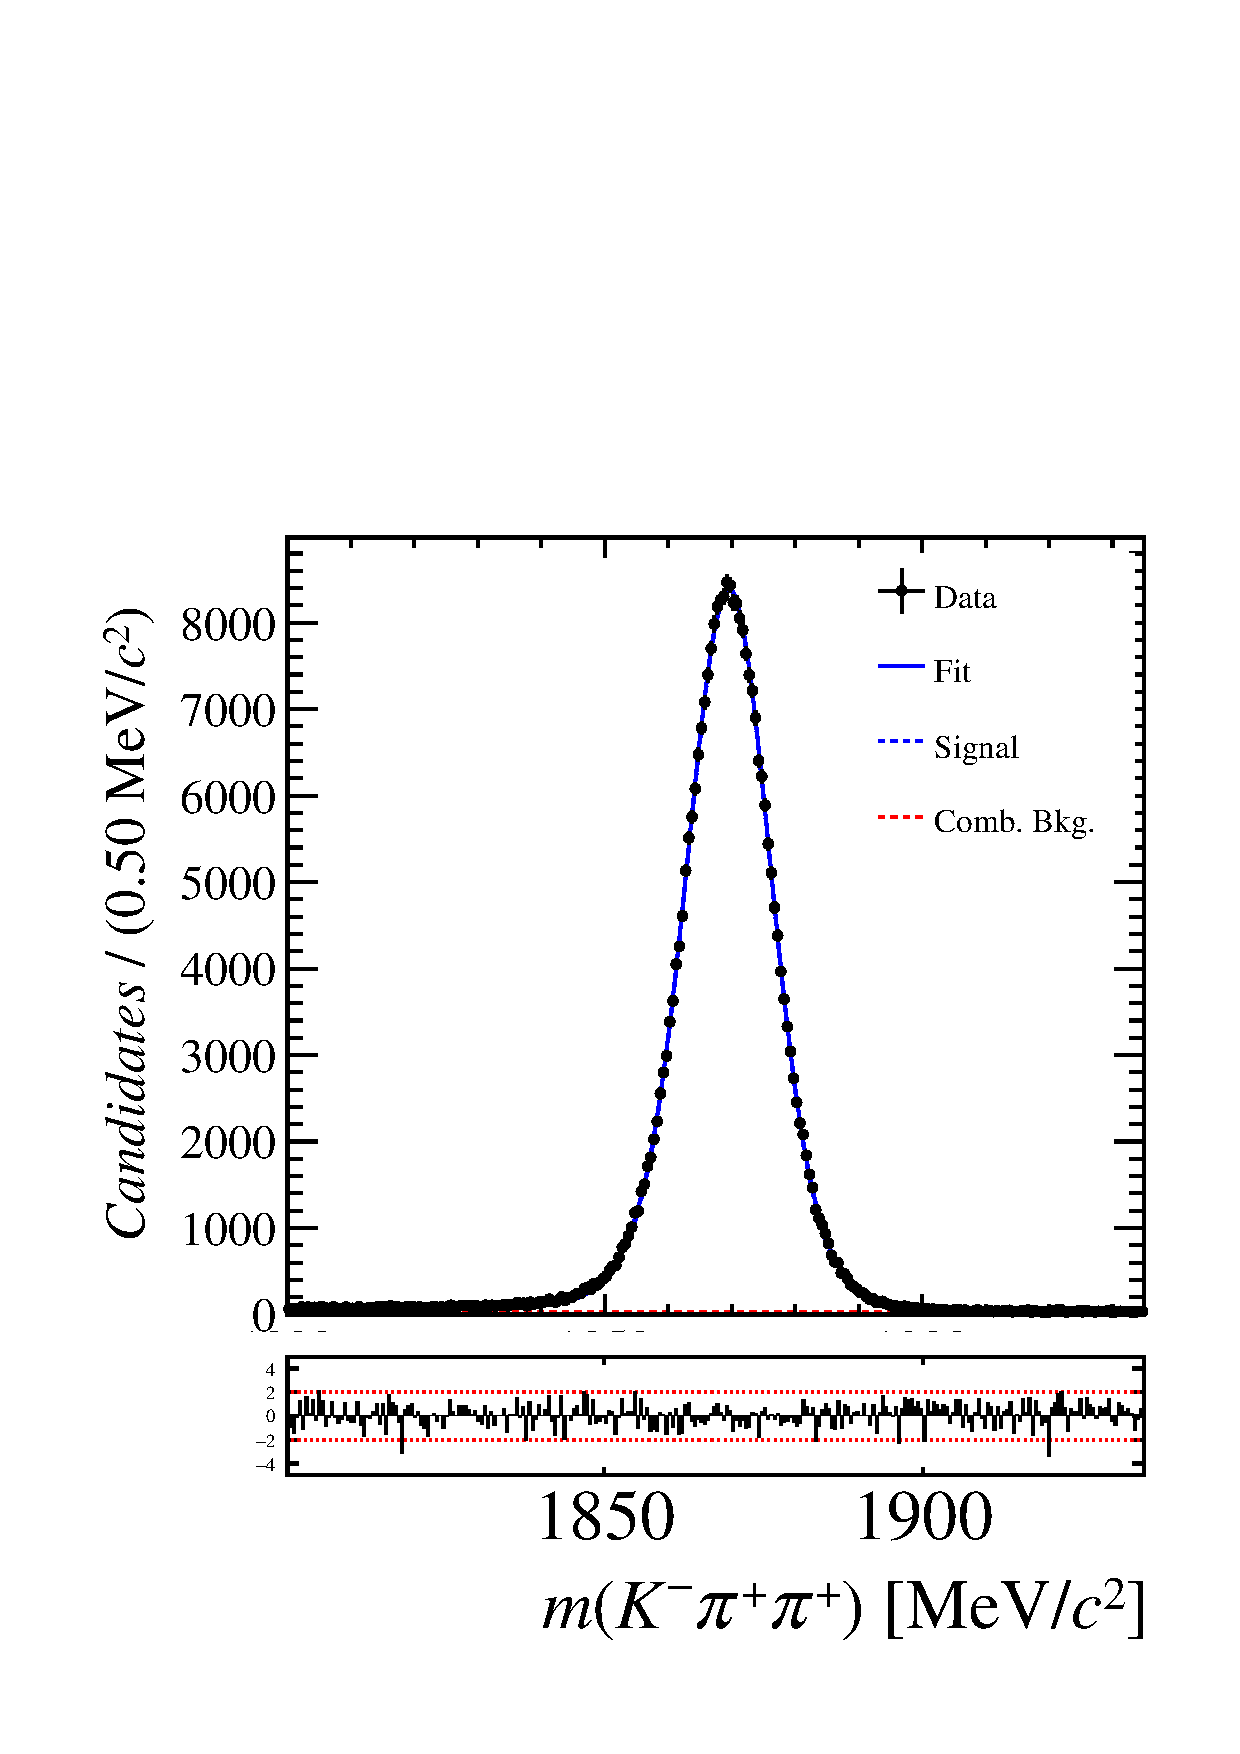
\includegraphics[height=5cm,width=0.4\textwidth]{figs/KpiAsym/fit_positive_kpipi_11up.pdf}\\
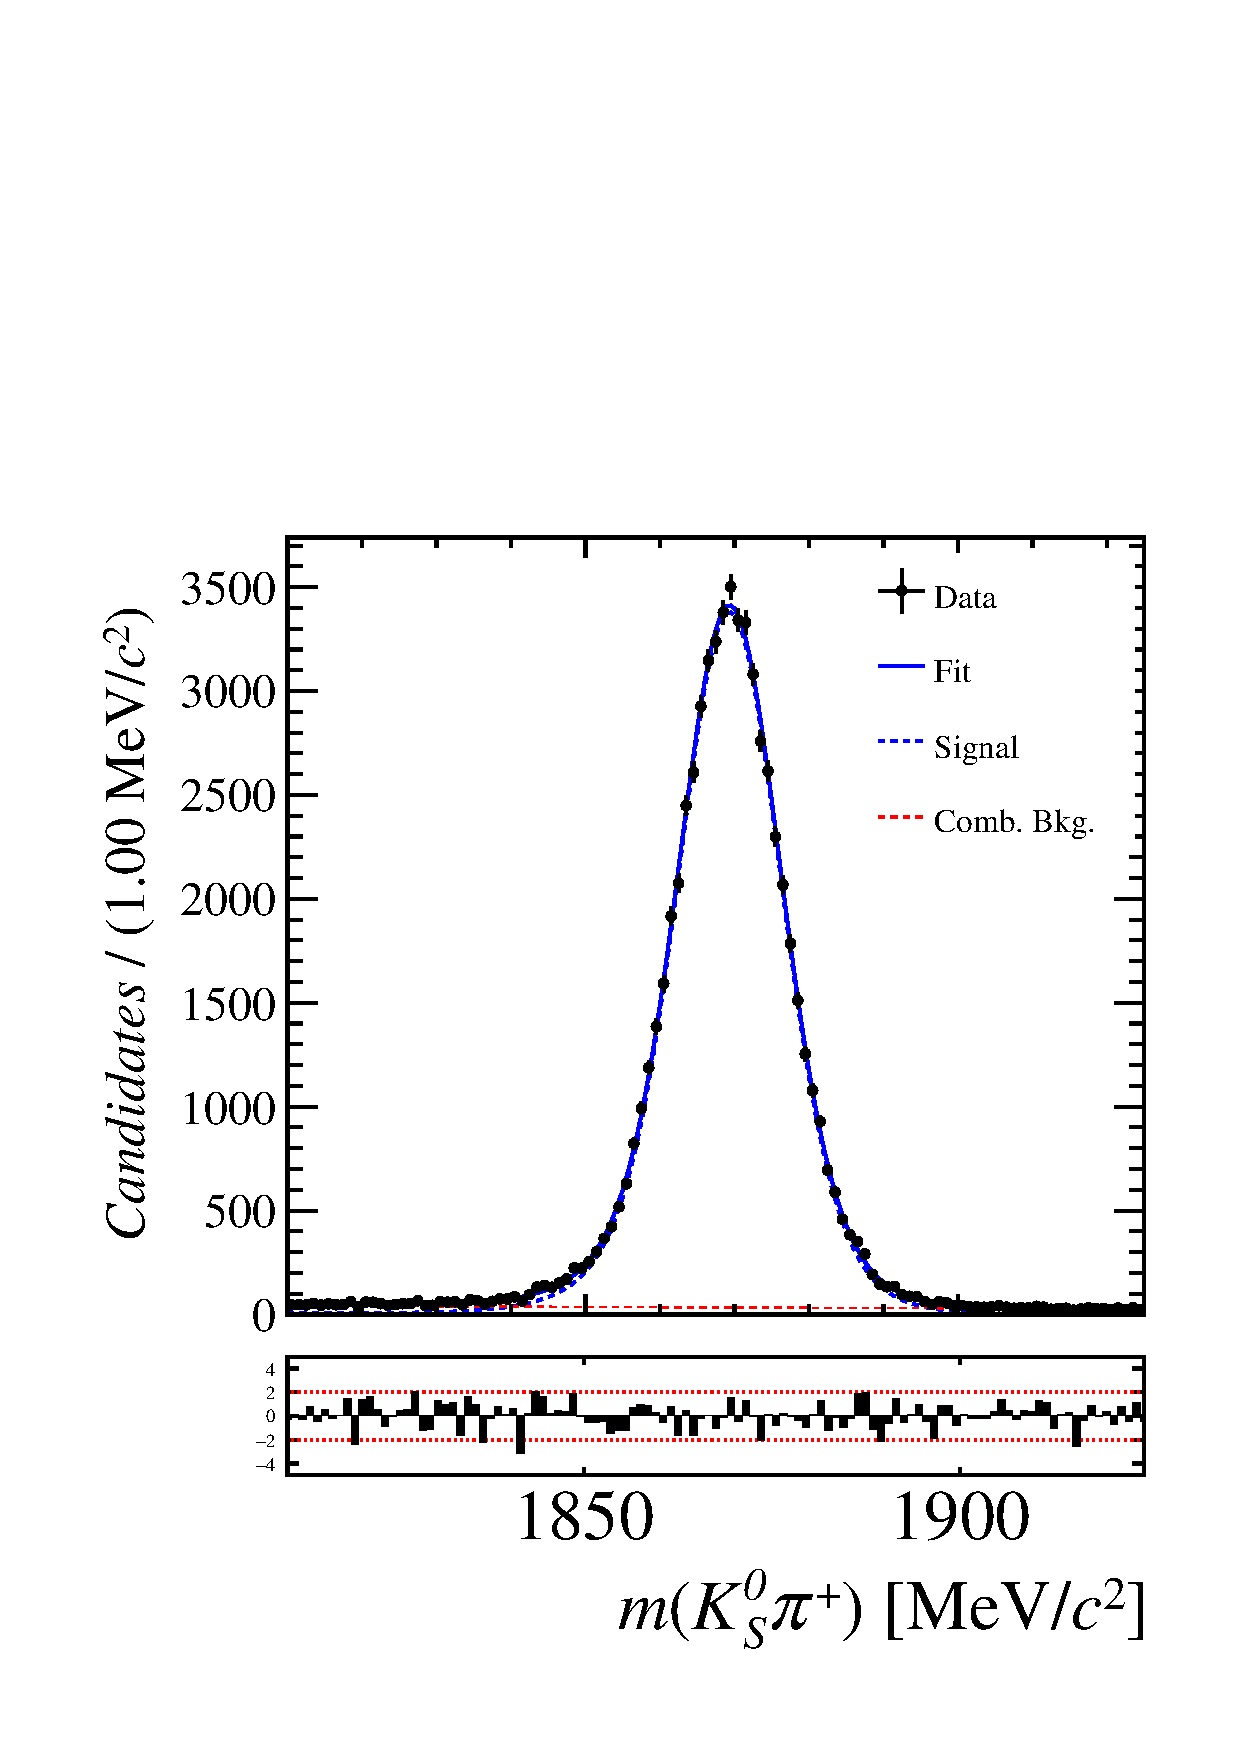
\includegraphics[height=5cm,width=0.4\textwidth]{figs/KpiAsym/fit_negative_kspi_11up.pdf}
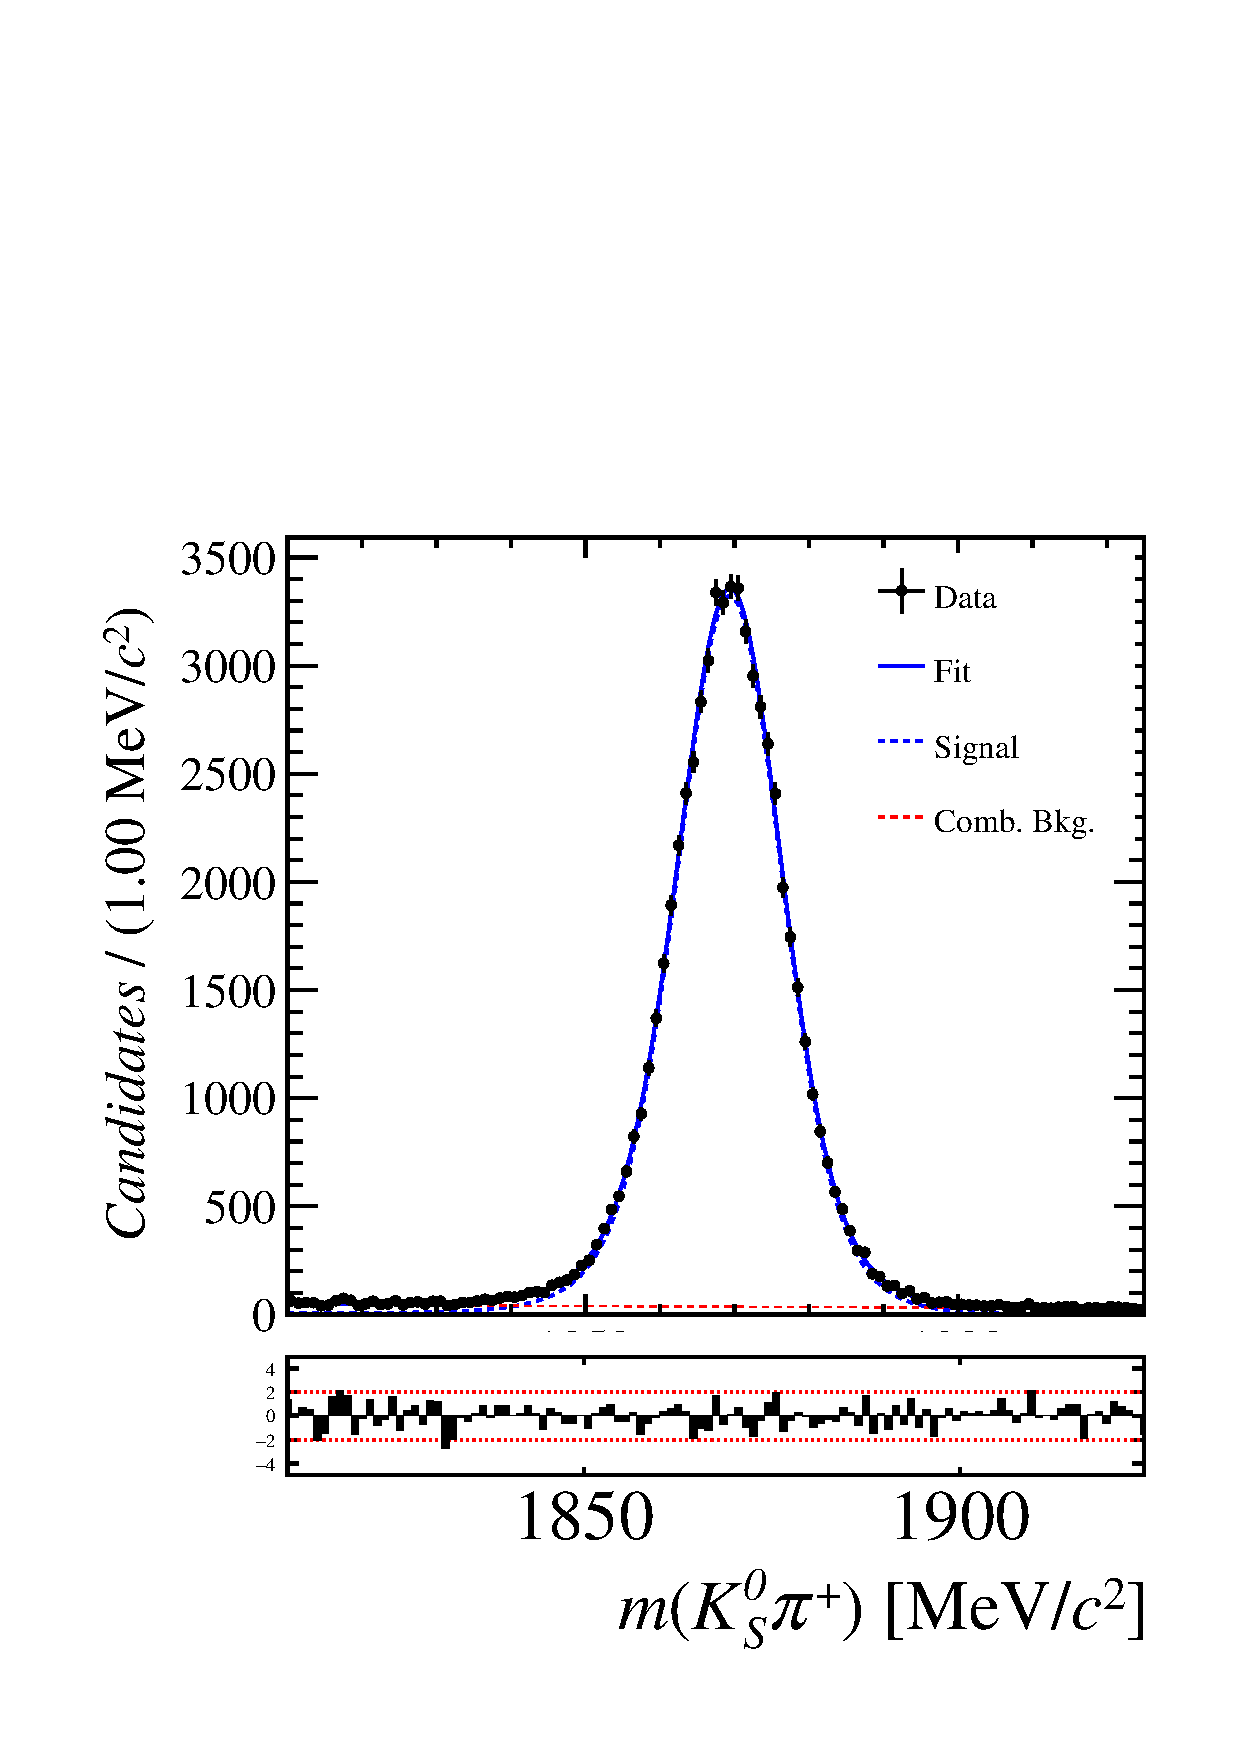
\includegraphics[height=5cm,width=0.4\textwidth]{figs/KpiAsym/fit_positive_kspi_11up.pdf}
\caption{Distributions of the invariant mass of (top) $\Dpm\to\Kpm\pipm\pipm$ and (bottom) $\Dpm\to\KS\pipm$ candidates for Run-I data from the calibration samples. A fit described in the text is overlaid.}
\label{fig:KpiAsymFitsRun1}
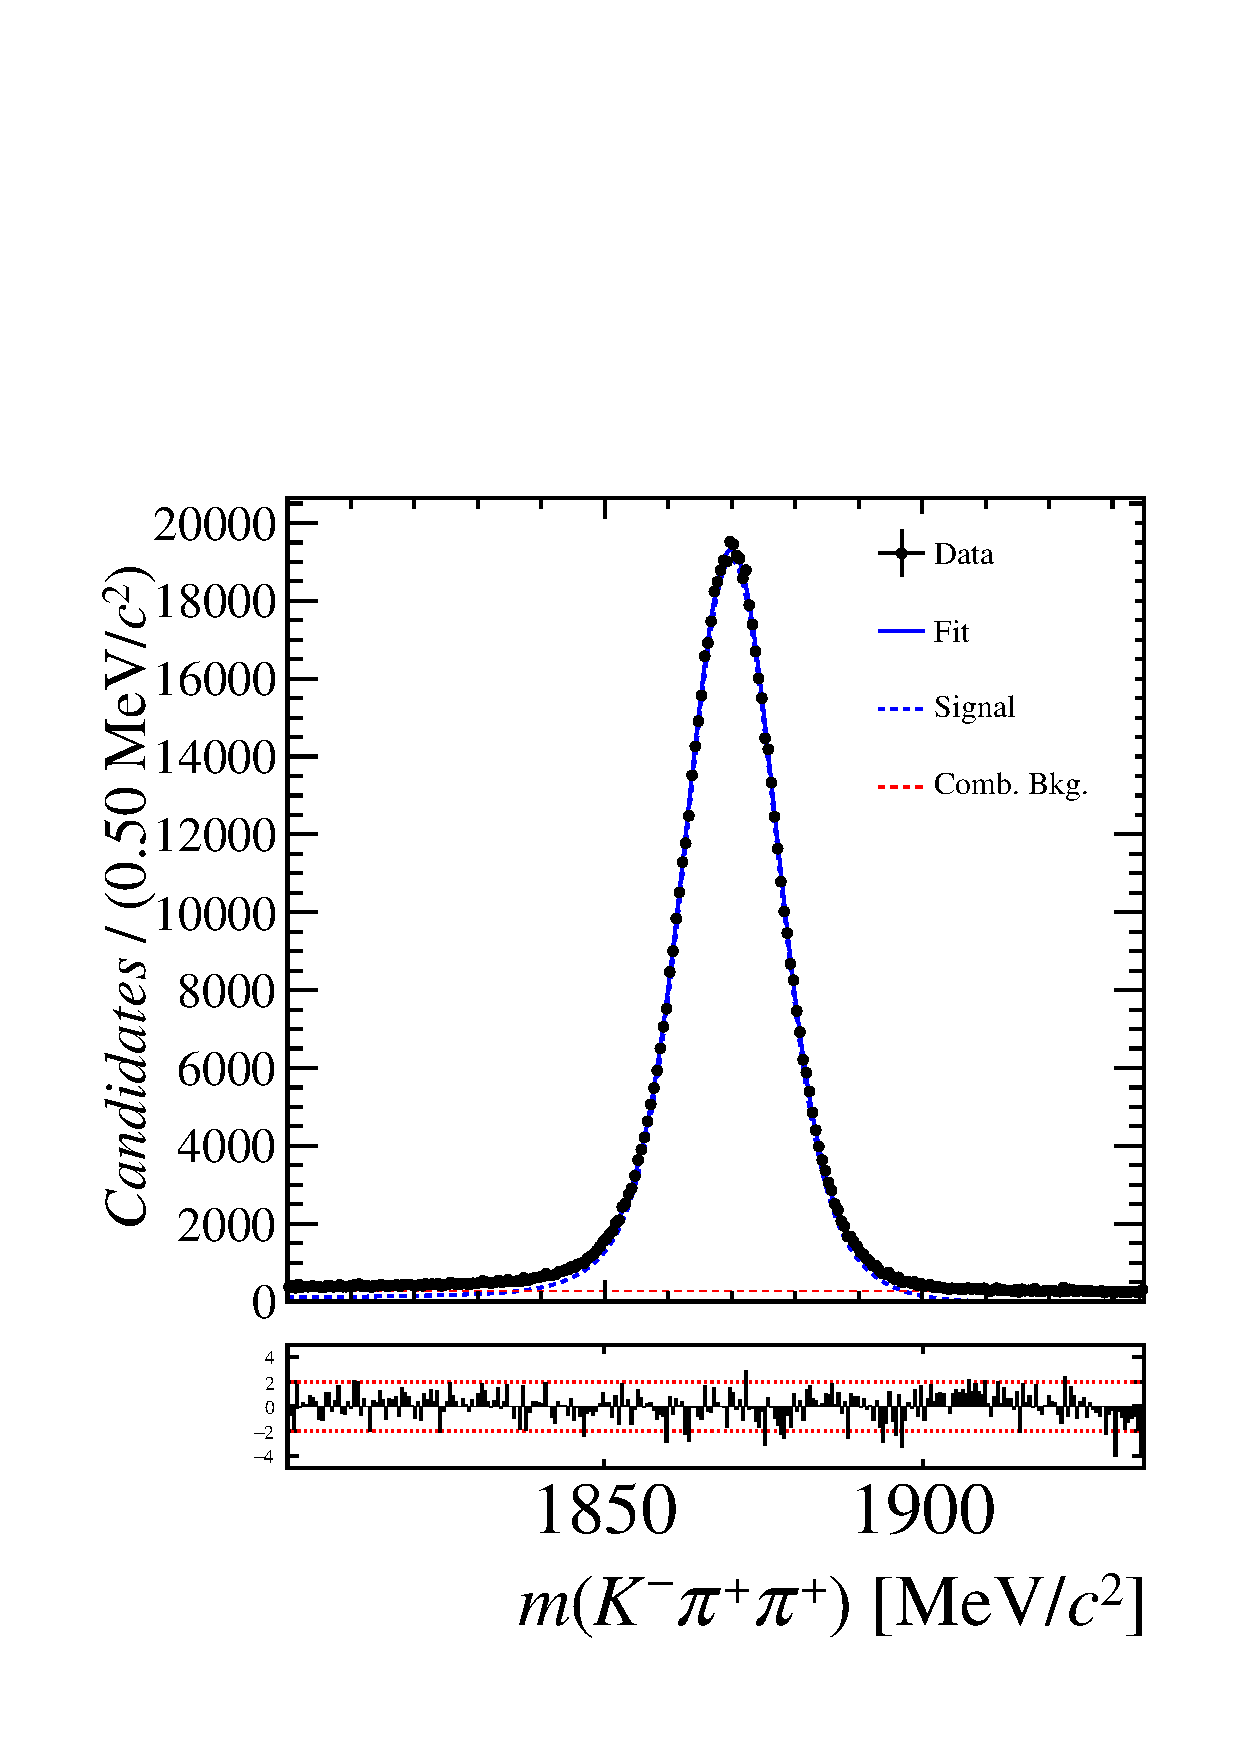
\includegraphics[height=5cm,width=0.4\textwidth]{figs/KpiAsym/fit_negative_kpipi_15up.pdf}
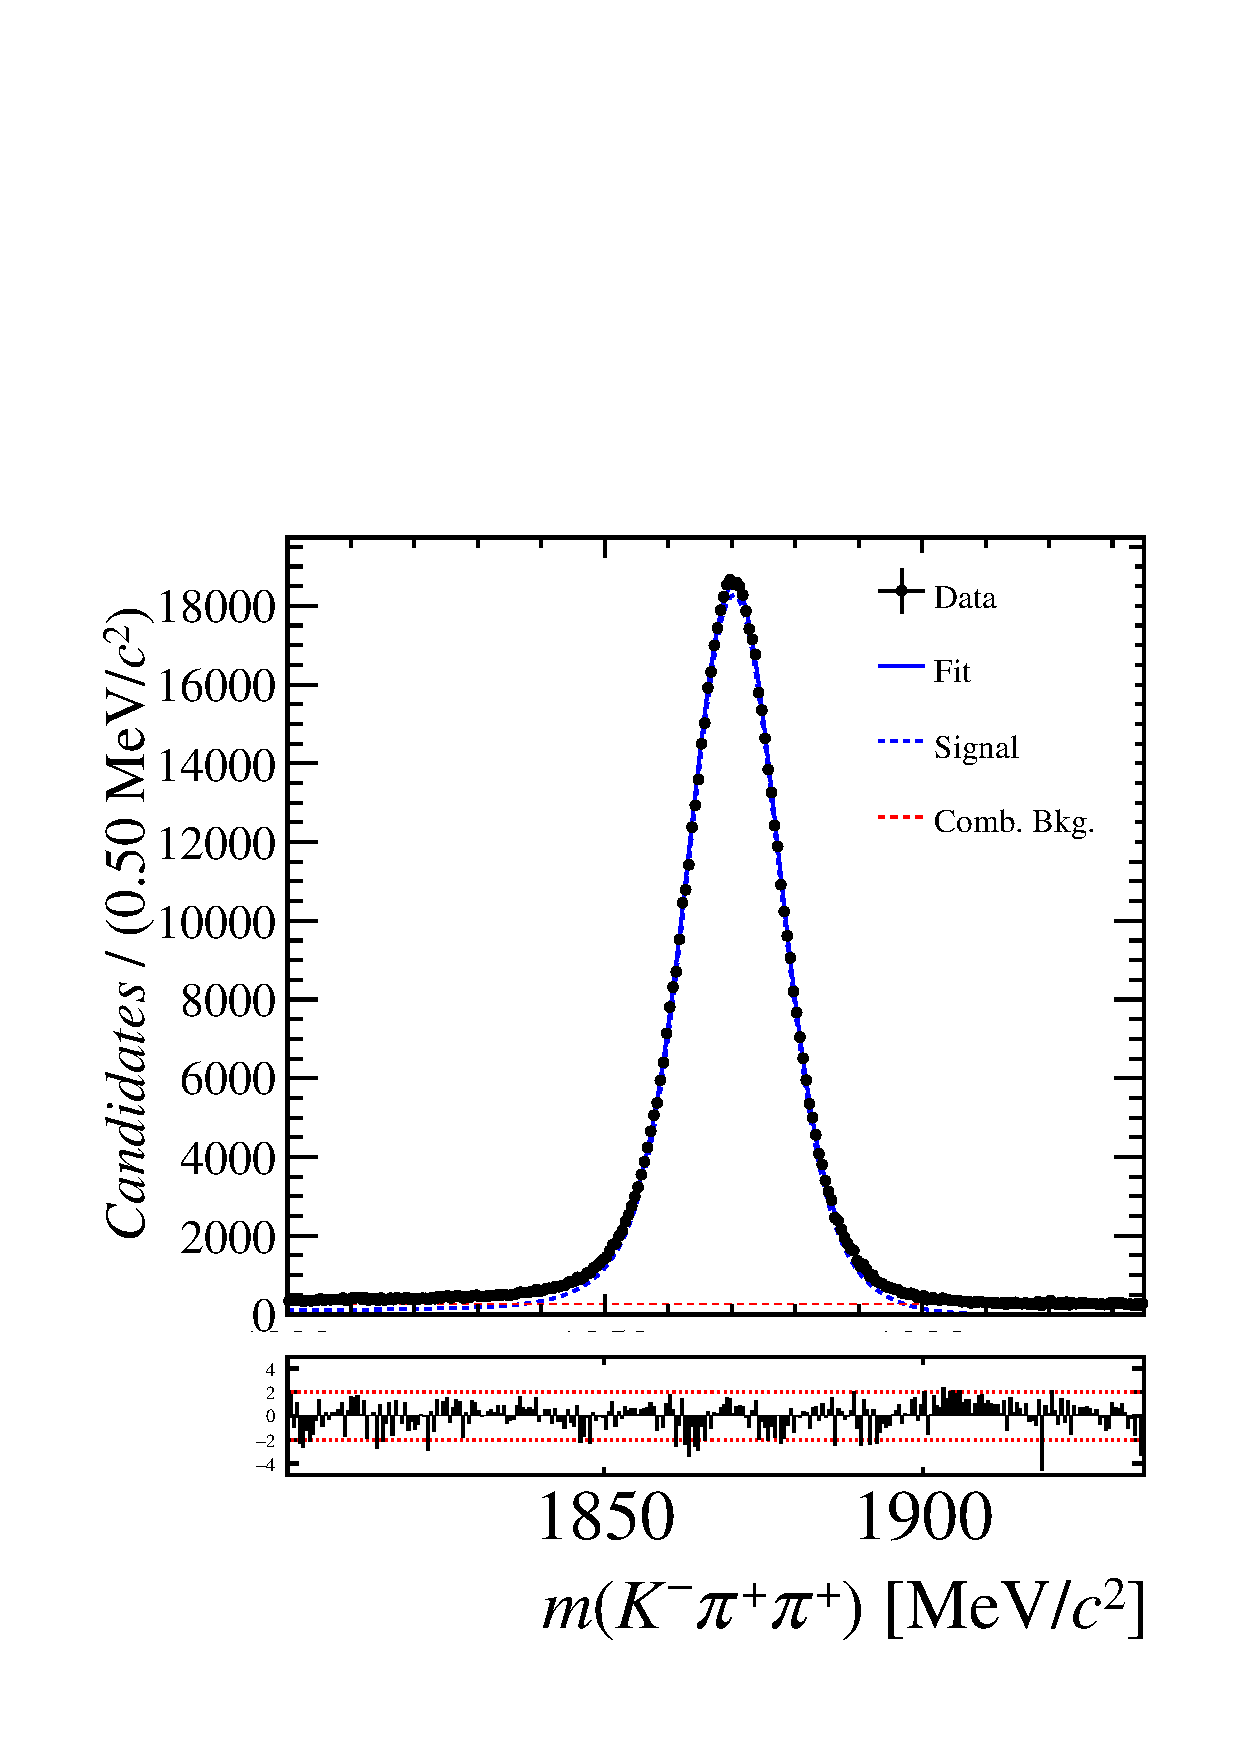
\includegraphics[height=5cm,width=0.4\textwidth]{figs/KpiAsym/fit_positive_kpipi_15up.pdf}\\
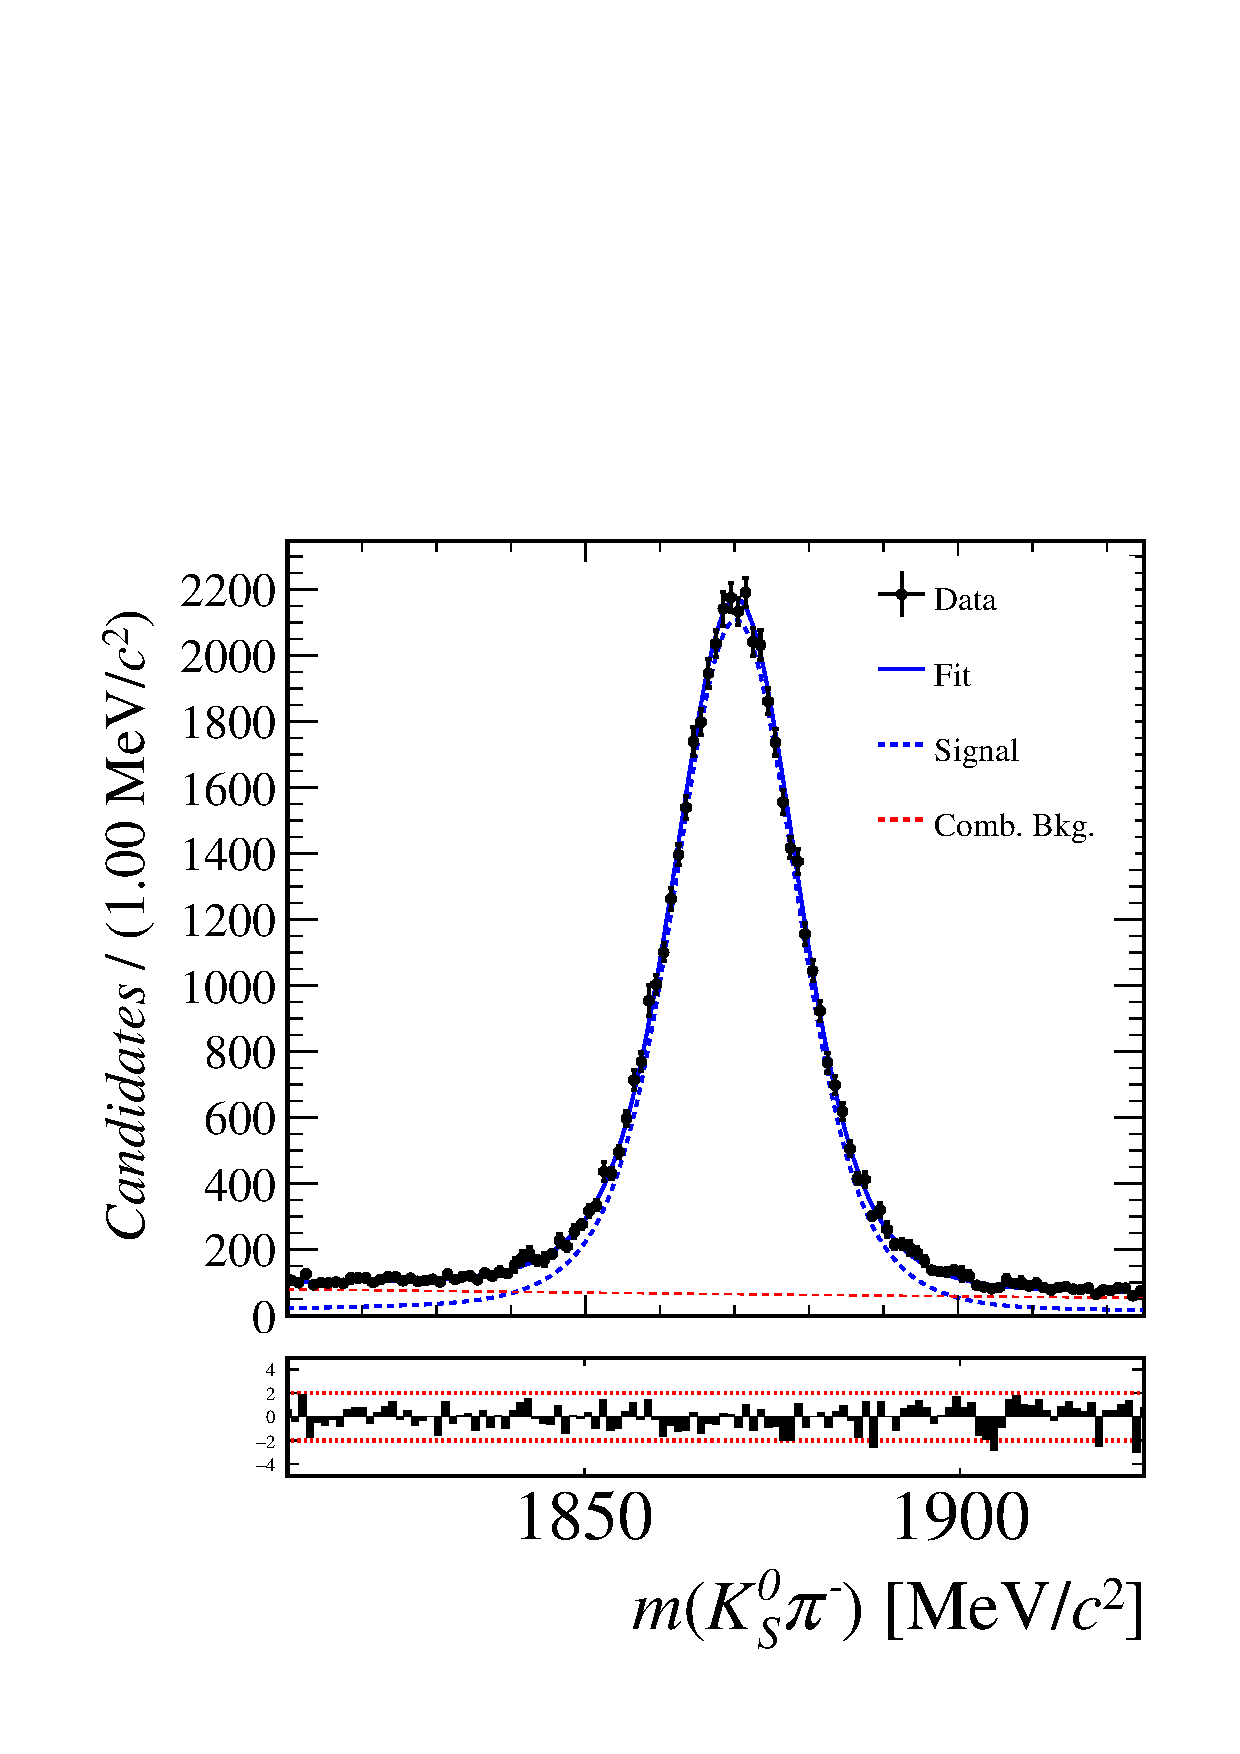
\includegraphics[height=5cm,width=0.4\textwidth]{figs/KpiAsym/fit_negative_kspi_15up.pdf}
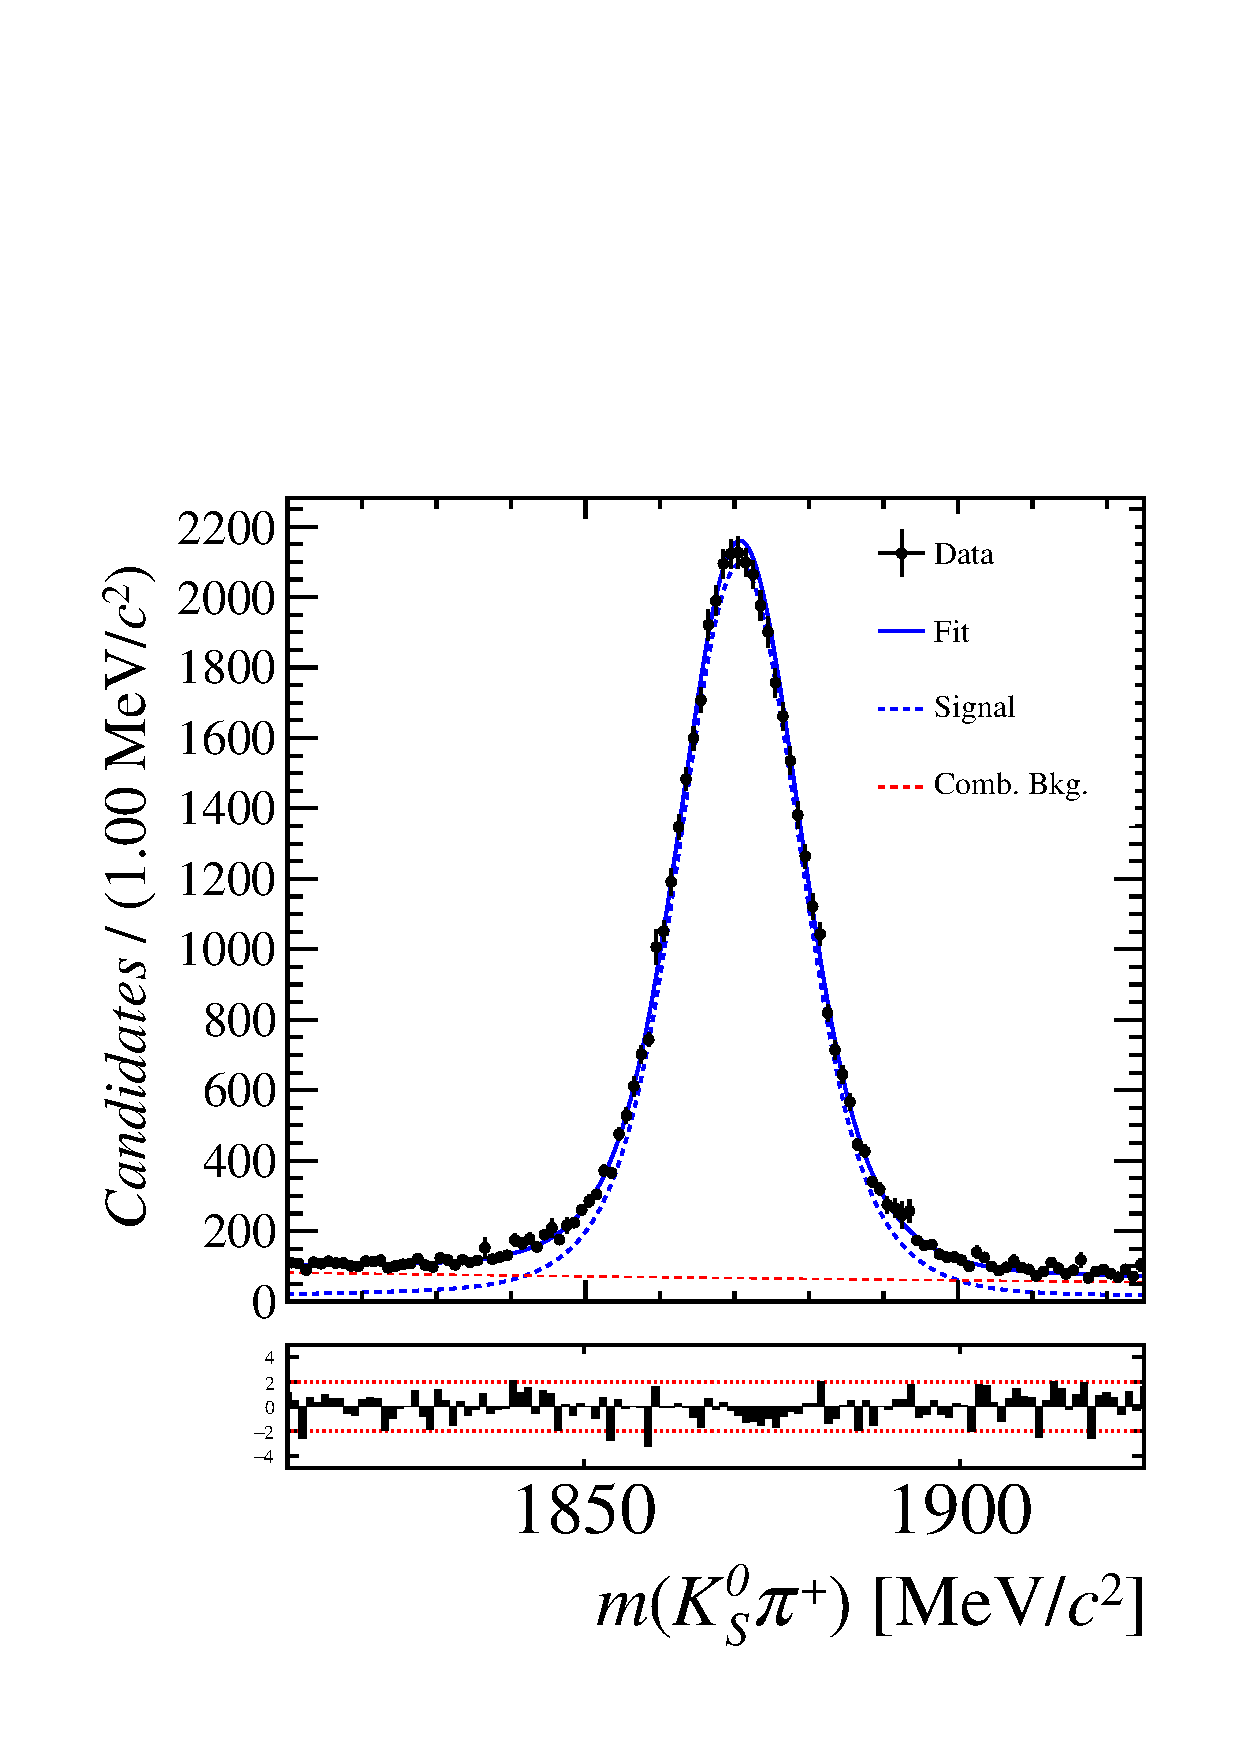
\includegraphics[height=5cm,width=0.4\textwidth]{figs/KpiAsym/fit_positive_kspi_15up.pdf}
\caption{Distributions of the invariant mass of (top) $\Dpm\to\Kpm\pipm\pipm$ and (bottom) $\Dpm\to\KS\pipm$ candidates for Run-II data from the calibration samples. A fit described in the text is overlaid.}
\label{fig:KpiAsymFitsRun2}
\end{figure}


\begin{table}[h]
\centering
 \begin{tabular}{l c}
 \hline
 \hline
Data sample & $A^{det}(\Km\pip)$ + $A(\Kz)$ [\%] \\
\hline
Run-I & \\ 
2011, mag. up & -2.01 $\pm$ 0.32\\
2011, mag. down &  -0.16 $\pm$  0.28\\
2011, average & -1.09 $\pm$ 0.21\\

2012, mag. up &  -0.90 $\pm$ 0.20\\
2012, mag. down & -1.01 $\pm$ 0.22 \\
2012, average & -0.96 $\pm$ 0.15\\
\\
Run-II & \\ 
mag. up & -1.16 $\pm$ 0.34 \\
mag. down & -0.65 $\pm$ 0.27 \\
average & -0.91 $\pm$ 0.22\\
%2016, mag. up &  0.50 $\pm$ 0.88\\
%2016, mag. down & 1.23 $\pm$ 0.72 \\
%2016, average & 0.87 $\pm$ 0.57\\
\hline
\hline
\end{tabular}
\caption{Summary of the $\Km\pip$ detection asymmetry obtained from the fits to the Run-I and Run-II calibration samples.}
\label{table:KpiDetectionAsym}
\end{table}

